\documentclass[a4paper,12pt]{article}

\usepackage[margin=1in]{geometry}
\usepackage{tikz}
\usepackage{amssymb}
\usepackage{xcolor}
\usepackage{circuitikz}
\usepackage{graphicx}

\newcommand{\ra}{$\rightarrow$}
\newenvironment{6mini}{
  \begin{minipage}{6cm}
}{
  \end{minipage}
}

\title{\texttt{Decoders}\\\hrulefill}
\author{Module 7}
\date{\small{10/2/2023}}

\begin{document}
    \maketitle

    \section{Active Inputs And Outputs}
      Logic device inputs and outputs can be active high or low.
        \begin{itemize}
          \item Active HIGH is when a 1 \texttt{activates} a given input, or output.
          \item Active LOW is when a 0 \texttt{activates} a given input, or output.
        \end{itemize}
    
    \section{Decoding}
      It's taking an input combination, which can be called a code, and translating it to one or more active ouputs. 
      \begin{itemize}
        \item BCD Decoder Decodes the BCD input to various outputs - BCD to 7 segment
        \item X of Y decoder (standard decoder)-Decodes input X to activate (only) one of the Y outputs.
      \end{itemize}
      \subsection{Standard Decoder}
        \begin{itemize}
          \item One output is active at a time. Active high refers to only one output being 1 at a time, while active low refers to only one being 0.
          \item number of outputs is $2^n$, n being the number of inputs. \\
          Its tytpical nomenclature is $<$number of inputs$>$ to $<$number of outputs$>$ (not including enable input) decoder.
          \item 3 to 8 decoder, 3 x 8 decoder
        \end{itemize}
        Most decoders are active low outputs which use active low enable.

        \subsubsection{2 x 4 decoder}
          \begin{itemize}
            \item if enable is not active, output is inactive
            \item only one output is active at a time
            \item Negation bubble on an enable, input, and an output indicates that it's an active low
          \end{itemize}

          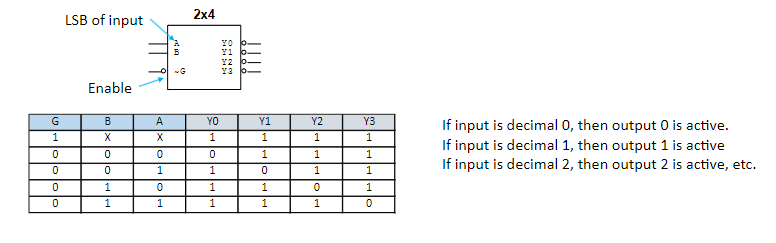
\includegraphics[width=20cm]{Two4Decoder.png}
          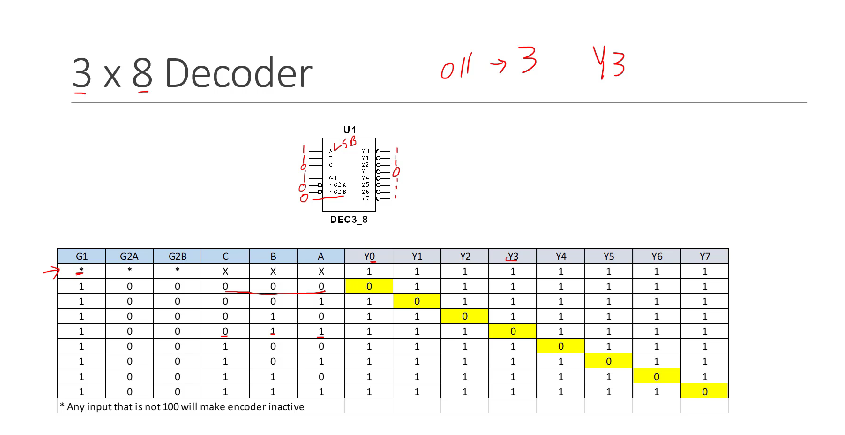
\includegraphics[width=20cm]{3x8decoder.png}
          \hrulefill

          \section{Cascading Decoders}
            Cascading another decoder will add 1 more input and double the output.
            \begin{itemize}
                \item Cascading 2x4 decoders will produce a 3x8 decoder
                \item Enable input becomes MSB of input of cascaded decoder
            \end{itemize}
            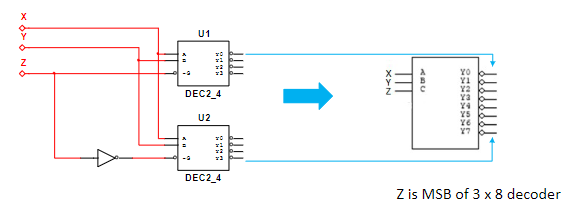
\includegraphics[width=15cm]{CascadingDecoder.png}\\
            The reason for having a not gate at the bottom enabler input, is that only one decoder is desired to be active at a time for any input combination. \vspace*{10pt}

            
            \begin{tabular}{ c c c } 
                \hline
                0 & 0 & 0 \\ 
                0 & 0 & 1 \\ 
                0 & 1 & 0 \\
                0 & 1 & 1 \\
                \underbar{~~~}&\underbar{~~~}&\underbar{~~~} \\
                1 & 0 & 0 \\
                1 & 0 & 1 \\
                1 & 1 & 0 \\
                1 & 1 & 1 \\
                \end{tabular}\\ \\
                The top Decoder takes the first half of the inputs, while the bottom takes the bottom half of the inputs
                \\ \includegraphics*[width=15cm]{CascadingDecoder2.png}

                \subsection{adding enables}
                  Whenever decoders are cascaded together, the enables are used to add a new input.
                  \begin{itemize}
                    \item for \texttt{active low enables} use an \textbf{OR} gate
                    \item for \texttt{active high enables} use an \textbf{AND} gate
                  \end{itemize}
                  \[X~\textnormal{AND}~1=X\] \[X~\textnormal{OR}~0=X\]
                  
                  \begin{figure}
                    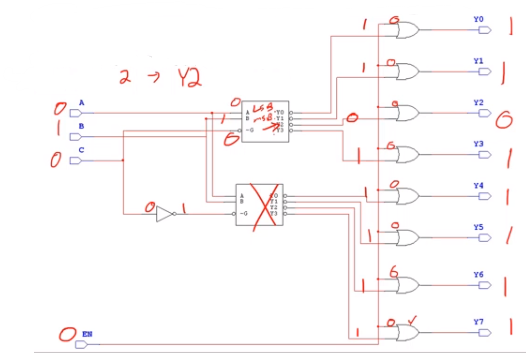
\includegraphics[width=10cm]{AddingEnables.png}
                    \caption{Example of adding active low enable}
                  \end{figure}
                
                \section{Using Decoders to Implement Minterms}  
                  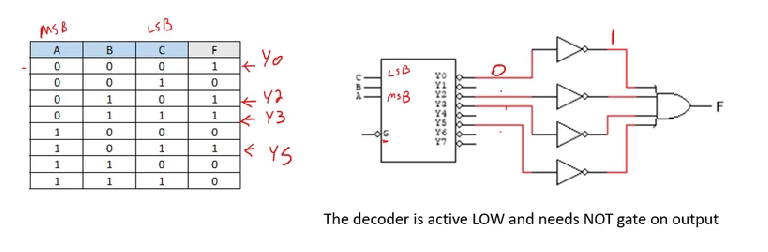
\includegraphics[width=15cm]{mintermDecoder.png}

                \section{Where Decoders are Used}
                  \subsection{Memory Addressing}
                    \begin{itemize}
                      \item Microprocessor needs to write to memory location
                      \item Microprocessor will send out binary code
                      \item Binary code determines which memory location should be active
                      \item Works the same for reading a memory location
                    \end{itemize}
                    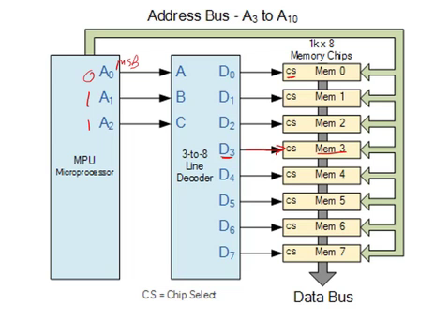
\includegraphics[width=10cm]{MemoryAdressing.png}

                  \subsection*{Selecting Sensors \& translating Binary Code}
\end{document}